%========================%
%        Preamble        %
%========================%
\documentclass[12pt]{amsart}

    %========================%
%        Packages        %
%========================%

\usepackage[utf8]{inputenc}
%\usepackage{amsmath}    % Included in amsart package
%\usepackage{amsthm}     % 
\usepackage{amssymb}      % 
\usepackage{mathtools}      % Paired Limiter Macros
% \usepackage{mdframed}       % boxes for theorem
\usepackage{enumitem}     % Continuous numbering of lists
\usepackage[hidelinks]{hyperref}
\usepackage{tikz}
\usetikzlibrary{positioning}
\usepackage{blindtext}
\usepackage{graphicx}
\usepackage{float}

%========================% 
%          Title         %
%========================% 
\title{Chapters 31 and 32 Notes}
\author{Anish Sundaram}
\date{\today}

%========================% 
%        Theorems        %
%========================% 
\theoremstyle{definition}
\newtheorem{theorem}{Theorem}  % Boxed theorems
\newtheorem{definition}{Definition} % Definitions
\newtheorem{example}{Example}       %
\newtheorem{algorithm}{Algorithm}
\newtheorem*{proof*}{Proof}         % non-numbered
\newtheorem*{remark}{Remark}        %
\numberwithin{equation}{theorem}    % Local equation numbering

\setcounter{tocdepth}{3}      % Show subsubsections in contents

%========================% 
%        Macros          %
%========================% 
\DeclarePairedDelimiter\abs{\lvert}{\rvert}  % Vertical bars
\DeclarePairedDelimiter\norm{\lVert}{\rVert} % Double vertical bars
\newcommand{\drawvec}[1]{                    % matrices on one line
    \begin{bmatrix}
        #1
    \end{bmatrix}
}


% \begin{figure}[H]
%     \centering
%     \includegraphics[width=5in]{global-carbon-cycle.png}
%     \caption{The Global Carbon Cycle}
%     \label{global-carbon-cycle}
% \end{figure}

%========================% 
%         Document       %
%========================% 
\begin{document}
\maketitle

\tableofcontents

\section*{31 Alternating Current}
In this chapter we will learn how resistors, inductors, and capacitors behave in circuits with sinusoidally varying voltages and currents. Many of the principles that we found useful in Chapter 30 are applicable, along with several new con- cepts related to the circuit behavior of inductors and capacitors. A key concept in this discussion is \textit{resonance}, which we studied in Chapter 14 for mechanical systems.


\subsection*{31.1 Phasors and Alternating Currents}

\begin{definition}
    \textbf{Alternating Current}:
    an electric current that reverses its direction many times a second at 
    regular intervals, typically used in power supplies. Alternating current has a peak voltage and current,
    as well as an average. Alternating current is provided by an \textbf{AC Source}
\end{definition}

\begin{definition}
    \textbf{Voltage Amplitude}:
    Because Voltage alternated due to fluctuation in AC current it has a sinusoidally
    shape, being described by the equation $$u = Vcos(\omega t)$$ where $u$ is the instantaneous
    potential difference and $V$ is the maximum or peak voltage, sometimes designated as $V_0$
    \begin{remark}
        In the US and Canada the common frequency for distribution systems is $f$ = 60Hz orr 377 rad/s, while
        the rest of the world uses $f$ = 50 Hz ($\omega$ = 314 rad/s)
    \end{remark}
\end{definition}

\begin{definition}
    \textbf{Angular Frequency($\omega$)}:
    Angular Frequency is a scalar measure of rotation rate. It refers to the rate of change of the argument of the sine function
    Angular Frequency can be found by the equation $$\omega = 2\pi f$$ where $f$ is the frequency measured in Hz.
\end{definition}

\begin{definition}
    \textbf{Current Amplitude}:
    Much like Voltage the Current outputted by an AC battery varies with time and fluctuates in a sinusoidal fashion which can be described by the equation $$i = Icos(\omega t)$$ where $i$ is instantaneous currnet and $I$ is peak current, sometimes designated as $I_0$
\end{definition}

\subsubsection*{31.1.1 Phasor Diagrams}

\begin{definition}
    \textbf{Phasors and Phasor Diagrams}:
    To represent sinusoidally varying voltages and currents, we use rotating vector diagrams wherein the instantaneous value is represented by the projection onto a horizontal axis of a vector with a length equal to the amplitude of the quantity which rotates CCW with angular speed $\omega$. These rotating vectors are called \textbf{Phasors}.
\end{definition}

\begin{figure}[H]
    \centering
    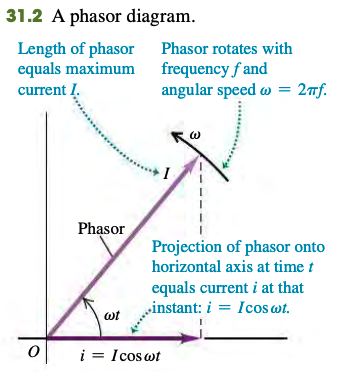
\includegraphics[width=3in]{Media/Phasor.png}
    \caption{Phase Diagram}
    \label{Phase Diagram}
\end{figure}

\subsubsection*{31.1.2 Recitified Alternating Current}

\begin{definition}
    \textbf{Rectified Average Current($I_{rav}$)}:
    Because it is dificult to measure alternating current in a Galvanometer we can use Recitified Average Current instead to measure. It can be computed by averaging the absolute value of a waveform over one full period of the waveform. or put into an equation as $$I_{rav} = \frac{2}{\pi}I = .637I$$ where $I$ is the current amplitude.
\end{definition}

\subsubsection*{31.1.3 Root-Mean-Squear(rms) Values}

\begin{definition}
    \textbf{RMS Current and Voltage}:
    Another more useful way to describe the current and voltage(which can be both positive or negative) is the root-mean-square value, of which is never 0 unless i/u is zero at every instant. RMS Current can be defined as $$I_{rms} = \frac{I}{\sqrt{2}}$$ and RMS Voltage can be defined as$$V_{rms} = \frac{V}{\sqrt{2}}$$ In other words dividing the peak value by $\sqrt{2}$.
\end{definition}

\subsection*{31.2 Resistance and Reactance}

\begin{definition}
    \textbf{Inductive Reactance($X_L$)}:
    Inductive reactance is the name given to the opposition to a changing current flow by an inductor, it is measured in Ohms like resistance. Inductive Reactance is calculated by the equation 
    $$X_L = 2\pi f L = \omega L$$ where $L$ is the inductance. The amplitude of voltage across an inductor for AC Current can be found by $$V_L = IX_L$$
    \begin{remark}
        The peaks of Inductor voltage and current are out of phase by a quarter-cycle. Since the voltage peaks occur a quarter-cycle earlier than the current peaks, we say that the voltage leads the current by 90°
    \end{remark}
\end{definition}

\begin{definition}
    \textbf{Capacitive Reactance($X_L$)}:
    Capacitive reactance is the name given to the opposition to a changing current flow by an Capacitor, it is measured in Ohms like resistance. Capacitive Reactance is calculated by the equation 
    $$X_C = \frac{1}{2\pi f L} = \frac{1}{\omega C}$$ where $C$ is the Capacitance. The amplitude of voltage across an Capacitor for AC Current can be found by $$V_L = IX_C$$
    \begin{remark}
        The peaks of Capacitor voltage and current are out of phase by a quarter-cycle. Since the voltage peaks occur a quarter-cycle before than the current peaks, we say that the voltage trails the current by 90°
    \end{remark}
\end{definition}

\begin{remark}
    Greater reactance leads to smaller currents for the same voltage applied. 
\end{remark}

\begin{definition}
    \textbf{Phase Angle ($\phi$)}:
    The Phase Angle represents the fraction of the period that y lags or leads the function. In our case it is the phase of the voltage relative to current.
    \begin{enumerate}
        \item For a pure Resistor $\phi = 0$
        \item For a pure Inductor $\phi = 90$
        \item For a pure Capacitor $\phi = -90$
    \end{enumerate}
   
    \begin{remark}
        If the Circuit is more Capacitive then Inductive the Phase angle will be negative, opposite holds true as well.
    \end{remark}
\end{definition}

\subsection*{31.3 The L-R-C Series Circuit}

\begin{definition}
    \textbf{Impedance($Z$)}:
    The Impedance of an AC circuit is the effective resistance of an electric circuit or component to alternating current, arising from the combined effects of ohmic resistance and reactance. The general equation for Impedence is  $$Z = \sqrt{R^2 + (X_l - X_c)^2}$$ where $R$ is Resistance, $X_L$ is Inductive Reactance and $X_C$ is Capacitive Reactance. This can be used to find the total Current through an L-R-C or any derivative circuit through the equation $$V = IZ$$

    \begin{remark}
        To Find the Phase Angle of an L-R-C series Circuit the equation following can be used:
        $$tan\phi = \frac{X_L- X_c}{R}$$
    \end{remark}
\end{definition}

\begin{figure}[H]
    \centering
    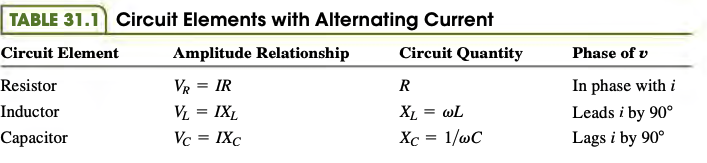
\includegraphics[width=5in]{Media/Elements.png}
    \caption{Phase rules of Circuit Elements}
    \label{Phase Rules of Circuit Elements}
\end{figure}

\subsection*{31.4 Power in AC Circuits}

\begin{remark}
    There is no power dissipated by a Capacitor or an Inductor as both absorb and release charge similar to a battery, and thus no power dissipates unlike a resistor.
\end{remark}

\begin{definition}
    \textbf{Average Power into a AC Circuit}:
    The average power into a general AC circuit can be calculated using the following equations:
    $$P_{aV} = .5VIcos\phi = V_{rms}I_{rms}cos\phi$$
\end{definition}

\begin{definition}
    \textbf{Power Factor}:
    The ratio of the actual electrical power dissipated by an AC circuit to the product of the r.m.s. values of current and voltage. The factor $cos\phi$ is called the power factor. 
\end{definition}

\subsection*{31.5 Resonance in AC Circuits}

\begin{definition}
    \textbf{Resonance}:
    The peaking of the current amplitude. The angular frequency $\omega_0$ at which the resonance peak occurs is called the \textbf{resonance angular frequency}. The Resonance Angular Frequency can be found by the equation $$\omega_0 = \frac{1}{\sqrt{LC}}$$
\end{definition}

\begin{definition}
    \textbf{Resonance Frequency ($f_0$)}:
     is when $X_L$ is equal to $X_C$. Resonance Frequency is found by the equation 
     $$f_0 = \frac{\omega_0}{2\pi} = \frac{1}{2\pi \sqrt{LC}}$$

     \begin{remark}
         When a circuit is at resonance frequency the inductive reactance and capacitive reactace are the same and thus negate eachother, so the only impedence comes from the resistor and the reactance is null.
     \end{remark}
\end{definition}

\subsection*{31.6 Tranformers}

    \begin{definition}
        \textbf{Transformers}:
        A transformer is used to transform the voltage and current levels in an ac circuit. In an ideal transformer with no energy losses, if the primary winding has N1 turns and the secondary winding has N2 turns, the amplitudes (or rms values) of the two voltages are related.
        The relations used by transformers are:
        $$\frac{V_2}{V_1} = \frac{N_2}{N_1}$$
        and
        $$V_1I_1 = V_2I_2$$
        and
        $$\frac{N_1}{N_2} = \frac{I_2}{I_1}$$
        For all of which 1 is the primary and 2 is the secondary.
    \end{definition}

\end{document}
